\documentclass[11pt,a4paper]{article}

\usepackage[margin=2.2cm]{geometry}
\usepackage{amsmath,amssymb,bm}
\usepackage{booktabs}
\usepackage{graphicx}
\usepackage{float}
\usepackage[table]{xcolor}
\usepackage{microtype}
\usepackage{enumitem}
\usepackage{fancyhdr}
\usepackage{hyperref}

\definecolor{oucblue}{RGB}{0,83,156}
\definecolor{lightblue}{RGB}{232,242,252}
\hypersetup{colorlinks=true,linkcolor=oucblue,urlcolor=oucblue,citecolor=oucblue}
\setlist{nosep,leftmargin=1.6em}
\setlength{\parindent}{0pt}
\setlength{\parskip}{0.55em}
\setlength{\headheight}{14pt}
\pagestyle{fancy}
\fancyhf{}
\lhead{LAB2: ROS Installation and Use}
\rhead{Li Yunzhe}
\cfoot{\thepage}
\renewcommand{\headrulewidth}{0.4pt}

\newcommand{\vect}[1]{\bm{#1}}
\newcommand{\R}{\mathbb{R}}

\begin{document}

\begin{titlepage}
  \centering
  \vspace*{2.2cm}
  {\color{oucblue}\rule{\textwidth}{1.2pt}}\\[1.2cm]
  {\Huge\bfseries LAB2: ROS Installation and Use\\[0.35cm]}
  {\Large Two-Drone Coordinate Frames, TF2, and Relative Motion}\par
  \vspace{1.1cm}
  {\color{oucblue}\rule{0.76\textwidth}{0.8pt}}\\[1.8cm]
  {\Large Visual Navigation for Autonomous Vehicles}\par
  \vspace{2.0cm}
  \begin{tabular}{rl}
    \textbf{Student:} & Li Yunzhe\\[0.25cm]
    \textbf{Institution:} & Ocean University of China\\[0.25cm]
    \textbf{Date:} & September 2026
  \end{tabular}
  \vfill
  {\large Experimental Report}
\end{titlepage}

\begin{abstract}
This experiment established a ROS Noetic development environment and implemented a two-drone rigid-transform scenario. A dynamic transform broadcaster generated the prescribed AV1 and AV2 poses at 50~Hz, while a TF2 listener recovered world-frame and relative-frame trajectories for RViz visualization. The catkin workspace compiled without warnings or failures. Runtime measurement gave a transform publication rate of 50.000~Hz. A synchronized 40-sample numerical test produced maximum errors of $2.220\times10^{-16}$ for the AV1 trajectory radius, $2.989\times10^{-16}$ for the AV2 world trajectory, $4.441\times10^{-16}$ for AV1 yaw, and $8.083\times10^{-16}$ for the relative position. The analytical derivation further shows that AV2 follows a parabola in the world $x_w$--$z_w$ plane and an ellipse on an oblique plane when observed from AV1. Quaternion operator identities and the equivalence between reversed intrinsic and extrinsic rotation sequences are also proved.
\end{abstract}

\section{Objectives}

The objectives were to understand the ROS computation graph, create and build a catkin workspace, inspect nodes and topics, publish time-varying coordinate transforms, query relative transforms through TF2, visualize rigid-body motion in RViz, and connect the observed trajectories to analytical rigid-transformation results. The assignment follows the MIT VNAV LAB2 specification~\cite{mitlab2}.

\section{Experimental Conditions}

The experiment used Ubuntu 20.04.6 LTS under WSL2, ROS Noetic with \texttt{roscore} version 1.17.4, catkin tools, TF2, RViz, and C++11. The software package contained one launch description, two C++ ROS nodes, a quadrotor mesh, an RViz configuration, and an independent transform-validation program. Table~\ref{tab:build} summarizes the final build and runtime checks.

\begin{table}[H]
\centering
\caption{Build and runtime verification.}
\label{tab:build}
\begin{tabular}{@{}ll@{}}
\toprule
Item & Observed result\\
\midrule
Catkin packages discovered & 1\\
Successful packages & 1\\
Build warnings / failures & 0 / 0\\
Dynamic TF publication rate & 50.000 Hz\\
Synchronized validation samples & 40\\
Numerical validation outcome & PASS\\
\bottomrule
\end{tabular}
\end{table}

\section{ROS and TF2 Design}

ROS separates a robotic application into independent nodes that exchange typed messages through topics. In the static scenario, two static-transform broadcasters publish the fixed poses of AV1 and AV2. The plotting node subscribes to the transform system and publishes visualization markers; RViz subscribes to the transform and marker topics. In the dynamic scenario, a single frame-publisher node replaces the two static broadcasters and publishes both time-stamped transforms on \texttt{/tf}. Figure~\ref{fig:graph} shows the implemented data flow.

\begin{figure}[H]
\centering
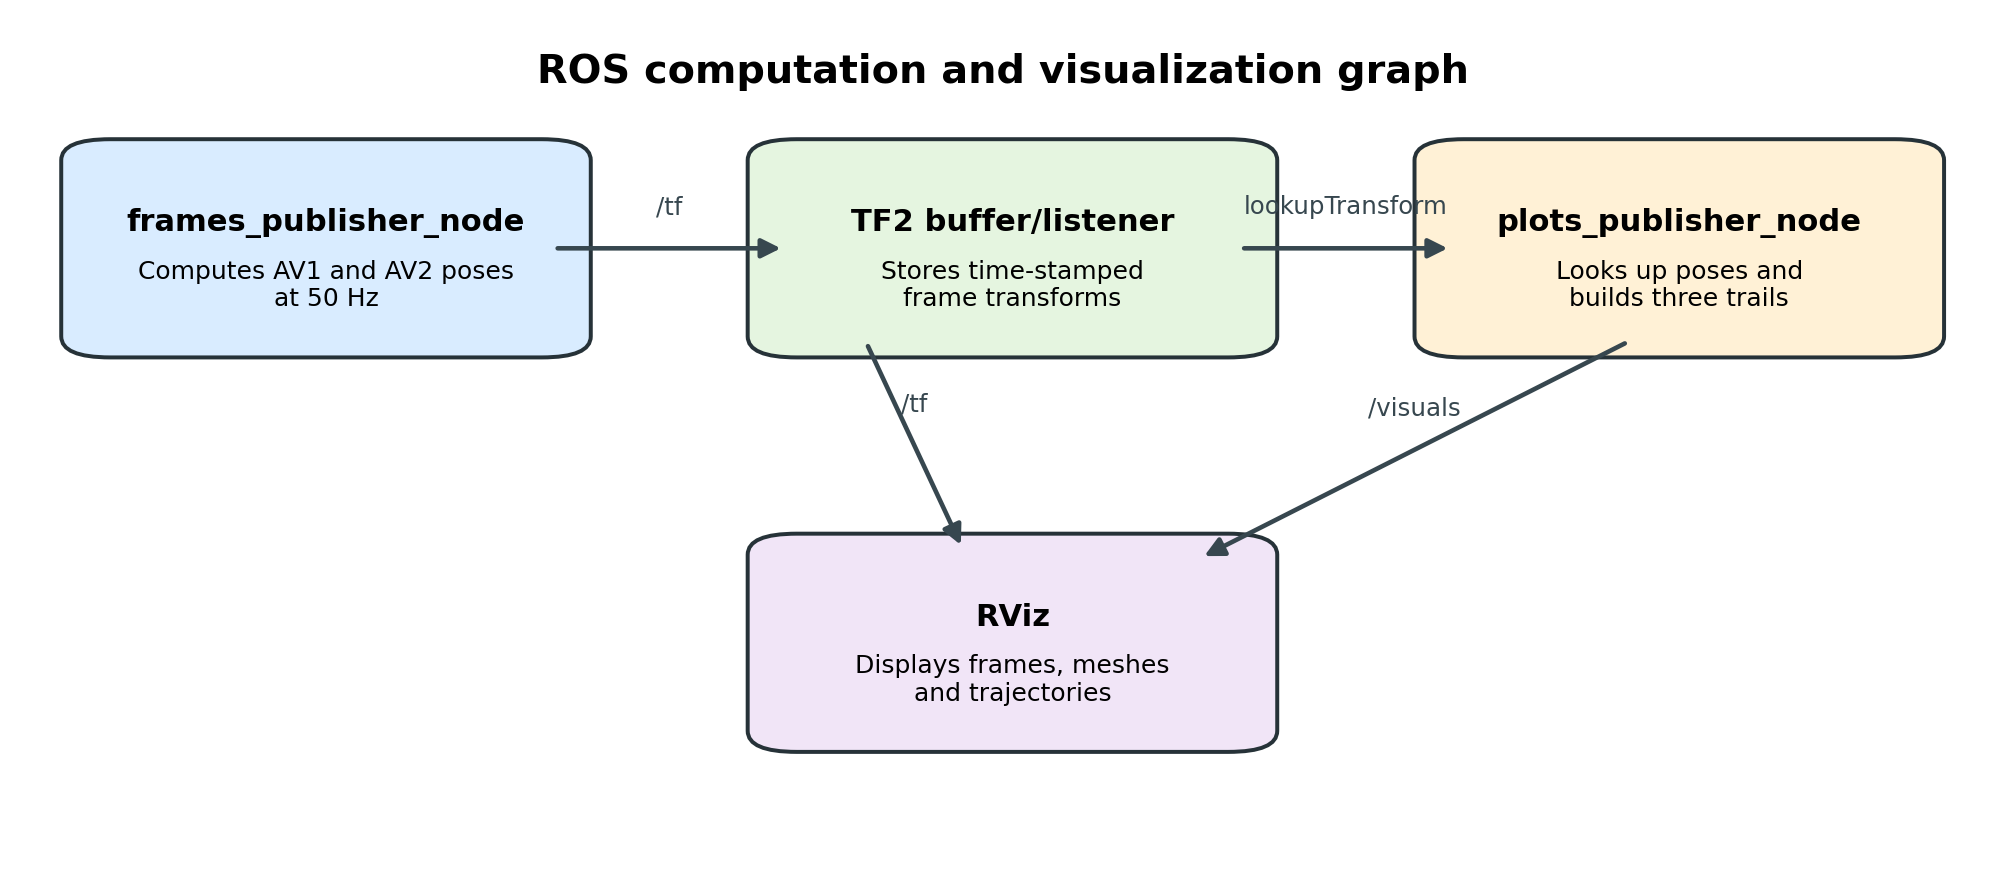
\includegraphics[width=0.95\textwidth]{figures/ros_system_graph.png}
\caption{ROS computation and visualization graph for the dynamic two-drone scenario.}
\label{fig:graph}
\end{figure}

TF2 represents every rigid transform with a parent frame, child frame, time stamp, translation, and unit quaternion. The broadcaster transmits a vector containing both drone transforms. The listener stores the transform history in a buffer, and the plotting node requests the latest transform from a selected reference frame to a destination frame. This design allows exactly the same physical pose to be viewed in either \texttt{world} or \texttt{av1} without changing the motion model. The published frame convention follows the standard ROS right-handed coordinate convention~\cite{rep103}, and the broadcaster interface follows the ROS TF2 API~\cite{tf2api}.

\subsection{Static scenario inspection}

Ignoring the logging node, the static configuration contained \texttt{av1broadcaster}, \texttt{av2broadcaster}, \texttt{plots\_publisher\_node}, and \texttt{rviz}. The static broadcasters published \texttt{/tf\_static}. The plotting node subscribed to \texttt{/tf} and \texttt{/tf\_static}, then published a \texttt{visualization\_msgs/MarkerArray} on \texttt{/visuals}. RViz subscribed to the two transform topics and \texttt{/visuals}. Therefore, the static broadcasters supplied the coordinate frames, while the plotting node supplied the two drone meshes and trajectory markers displayed by RViz.

When the static argument is omitted, its default value is false. The launch condition therefore suppresses the static-broadcaster group and enables the dynamic frame-publisher node. The \texttt{if} condition activates the fixed transforms only in static mode, whereas \texttt{unless} activates dynamic motion only when static mode is false.

\section{Dynamic Motion Implementation}

Let $t$ be the elapsed time after the frame-publisher node starts. The required world-frame positions are
\begin{equation}
\vect{o}_1^w(t)=
\begin{bmatrix}\cos t\\ \sin t\\0\end{bmatrix},
\qquad
\vect{o}_2^w(t)=
\begin{bmatrix}\sin t\\0\\\cos 2t\end{bmatrix}.
\label{eq:world_positions}
\end{equation}
AV1 has zero roll and pitch and yaw $t$, so its orientation is $R_z(t)$. This aligns its $y_1$ axis with the tangent of the unit circle while keeping $z_1$ parallel to $z_w$. AV2 undergoes pure translation and retains the identity orientation. A timer triggers publication every 0.02~s, giving the required 50~Hz rate.

The plotting node performs three transform lookups: AV1 in the world frame, AV2 in the world frame, and AV2 in the AV1 frame. The first two trails are solid world-frame curves. The third is a dashed relative-motion curve whose reference frame is AV1. RViz displays the coordinate axes, mesh markers, and all three trails.

\begin{figure}[H]
\centering
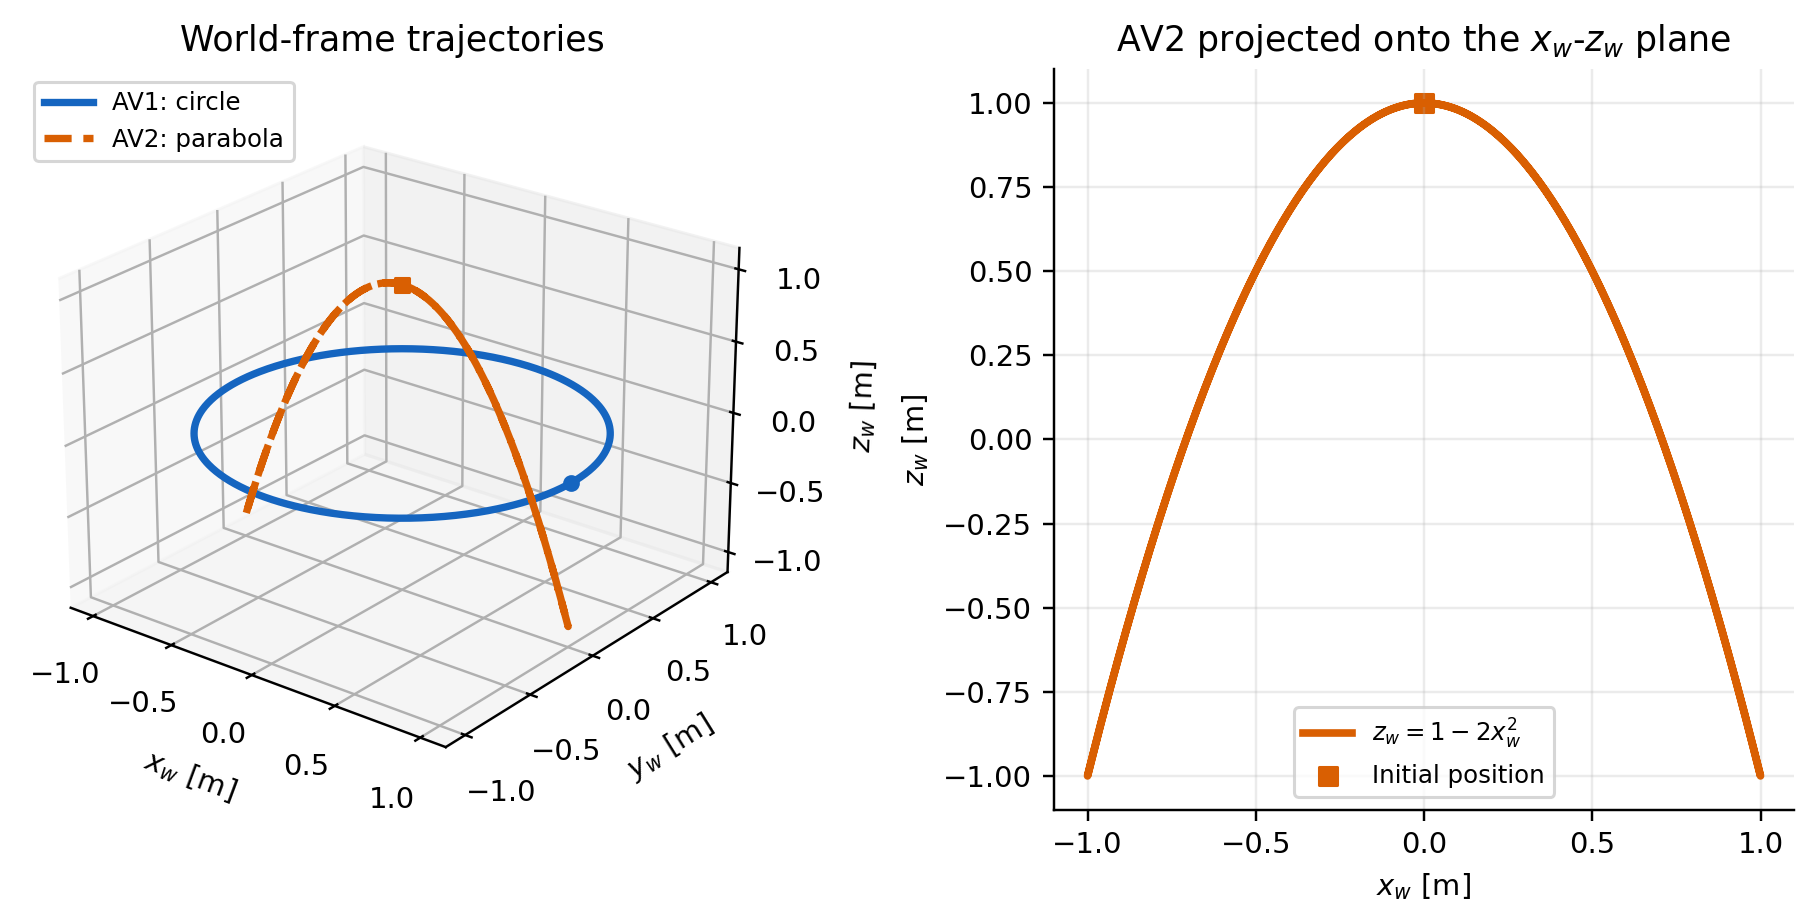
\includegraphics[width=0.96\textwidth]{figures/world_trajectories.png}
\caption{Analytical world-frame trajectories used to verify the dynamic ROS visualization. Color and line style both distinguish the two drones.}
\label{fig:world}
\end{figure}

\section{Runtime Results}

The dynamic computation graph contained \texttt{frames\_publisher\_node}, \texttt{plots\_publisher\_node}, and \texttt{rviz}, in addition to the ROS logging node. The frame publisher had no subscribers and published \texttt{/tf}. Both the plotting node and RViz subscribed to \texttt{/tf}; RViz also subscribed to \texttt{/visuals}. The measured transform rate was 50.000~Hz over the final observation window.

An independent validator sampled synchronized transforms at identical time stamps. For each sample it checked four invariants: $\sqrt{x_1^2+y_1^2}=1$, the AV2 position from Equation~\eqref{eq:world_positions}, AV1 yaw equal to $t$, and the complete AV2 position expressed in AV1. The acceptance tolerance was $10^{-3}$. Every measured error was more than twelve orders of magnitude below this limit, as shown in Table~\ref{tab:errors} and Figure~\ref{fig:validation}.

\begin{table}[H]
\centering
\caption{Maximum errors from 40 synchronized transform samples.}
\label{tab:errors}
\begin{tabular}{@{}lcc@{}}
\toprule
Checked quantity & Maximum error & Limit\\
\midrule
AV1 unit-circle radius & $2.220\times10^{-16}$ & $10^{-3}$\\
AV2 world trajectory & $2.989\times10^{-16}$ & $10^{-3}$\\
AV1 yaw & $4.441\times10^{-16}$ rad & $10^{-3}$ rad\\
AV2 position in AV1 & $8.083\times10^{-16}$ m & $10^{-3}$ m\\
\bottomrule
\end{tabular}
\end{table}

\begin{figure}[H]
\centering
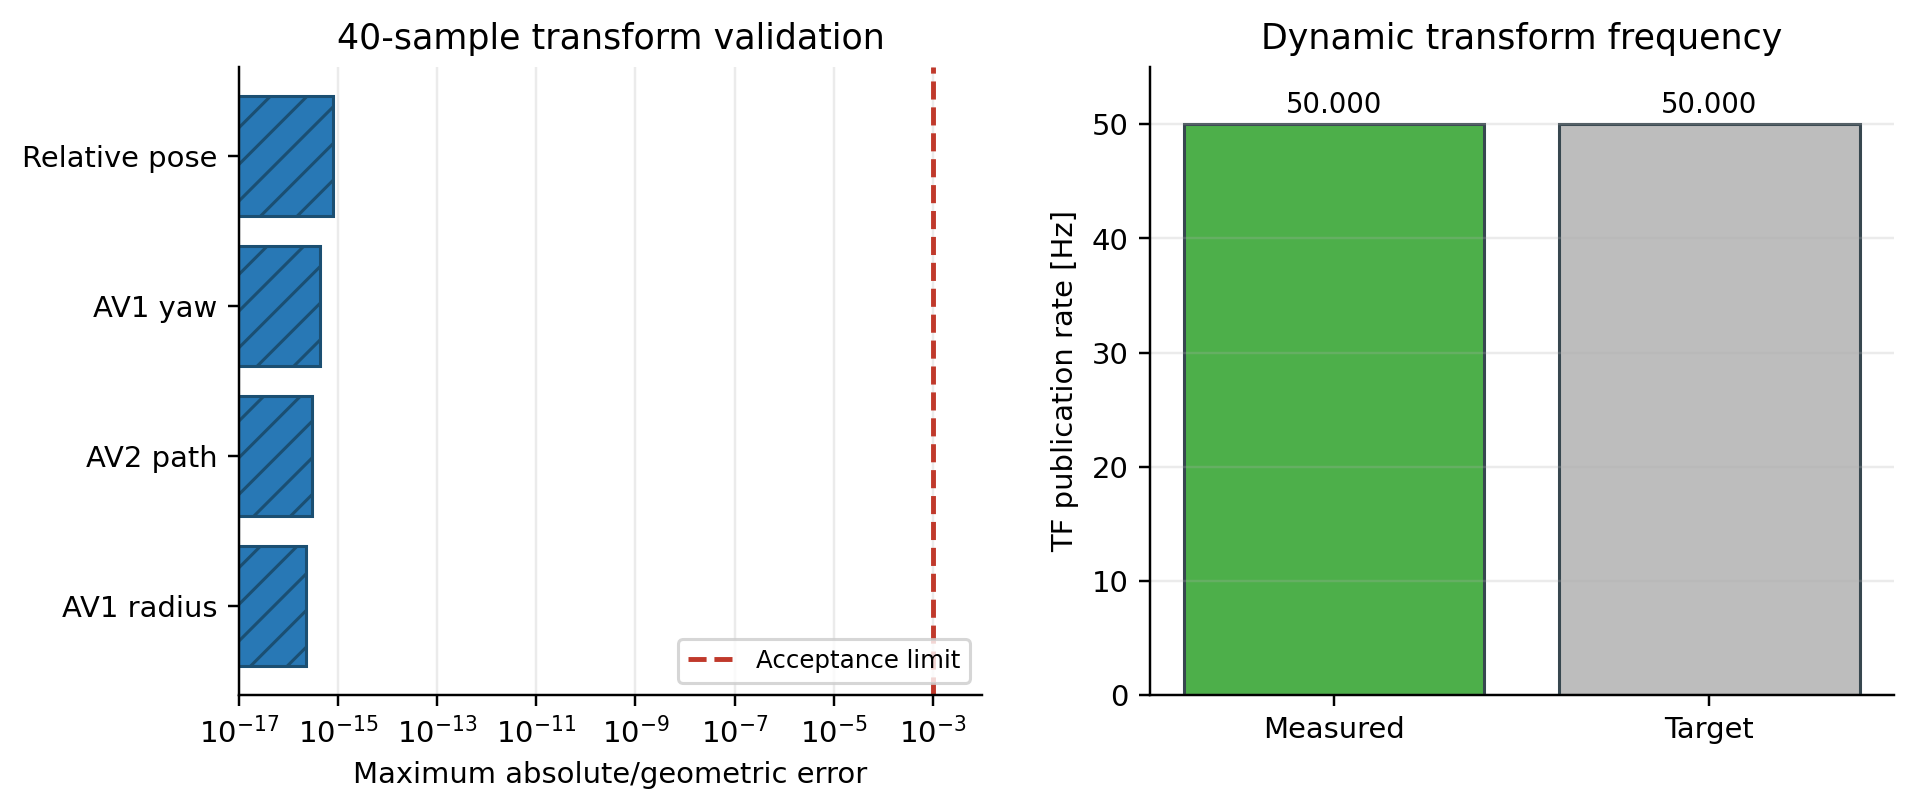
\includegraphics[width=0.94\textwidth]{figures/validation_summary.png}
\caption{Numerical transform errors and measured publication frequency.}
\label{fig:validation}
\end{figure}

\section{Rigid-Transformation Derivation}

\subsection{AV2 is a parabola in the world frame}

From Equation~\eqref{eq:world_positions}, $x_2^w=\sin t$, $y_2^w=0$, and $z_2^w=\cos 2t$. Applying $\cos 2t=1-2\sin^2t$ eliminates time:
\begin{equation}
y_2^w=0,\qquad z_2^w=1-2(x_2^w)^2.
\end{equation}
Thus AV2 lies in the world $x_w$--$z_w$ plane and follows the arc of a downward-opening parabola for $x_2^w\in[-1,1]$.

\subsection{AV2 expressed in the AV1 frame}

The homogeneous transforms from the two body frames to the world frame are
\begin{equation}
T_1^w=
\begin{bmatrix}
R_z(t)&\vect{o}_1^w\\\vect{0}^{\mathsf T}&1
\end{bmatrix},
\qquad
T_2^w=
\begin{bmatrix}
I_3&\vect{o}_2^w\\\vect{0}^{\mathsf T}&1
\end{bmatrix}.
\end{equation}
Therefore
\begin{equation}
T_2^1=(T_1^w)^{-1}T_2^w
=
\begin{bmatrix}
R_z(-t)&R_z(-t)(\vect{o}_2^w-\vect{o}_1^w)\\
\vect{0}^{\mathsf T}&1
\end{bmatrix}.
\end{equation}
With $c=\cos t$ and $s=\sin t$, the relative position becomes
\begin{align}
\vect{o}_2^1(t)
&=
\begin{bmatrix}c&s&0\\-s&c&0\\0&0&1\end{bmatrix}
\begin{bmatrix}s-c\\-s\\\cos 2t\end{bmatrix}\\
&=
\begin{bmatrix}cs-1\\-s^2\\\cos 2t\end{bmatrix}.
\label{eq:relative_position}
\end{align}

\subsection{Plane and centered coordinates}

Equation~\eqref{eq:relative_position} gives $y_2^1=-s^2$ and $z_2^1=1-2s^2$, hence
\begin{equation}
\Pi:\quad 2y_2^1-z_2^1+1=0.
\label{eq:plane}
\end{equation}
The relative trajectory is therefore planar. Place the new origin at
$\vect{p}^{,1}=(-1,-\tfrac12,0)^{\mathsf T}$ and choose the orthonormal basis
\begin{equation}
\vect{e}_{x_p}=\begin{bmatrix}1\\0\\0\end{bmatrix},\quad
\vect{e}_{y_p}=\frac{1}{\sqrt5}\begin{bmatrix}0\\1\\2\end{bmatrix},\quad
\vect{e}_{z_p}=\frac{1}{\sqrt5}\begin{bmatrix}0\\-2\\1\end{bmatrix}.
\end{equation}
The last vector is normal to $\Pi$. Projecting $\vect{o}_2^1-\vect{p}^{,1}$ onto this basis yields
\begin{equation}
x_p=\frac12\sin 2t,\qquad
y_p=\frac{\sqrt5}{2}\cos 2t,\qquad
z_p=0.
\label{eq:plane_coordinates}
\end{equation}
Eliminating $t$ gives
\begin{equation}
\frac{x_p^2}{(1/2)^2}+\frac{y_p^2}{(\sqrt5/2)^2}=1.
\end{equation}
Thus AV2 follows an ellipse centered at $\vect{p}^{,1}$ on the plane $\Pi$. Its semi-axis lengths are $1/2$~m and $\sqrt5/2$~m. Figure~\ref{fig:relative} shows the same curve in AV1 coordinates and in the centered plane frame.

\begin{figure}[H]
\centering
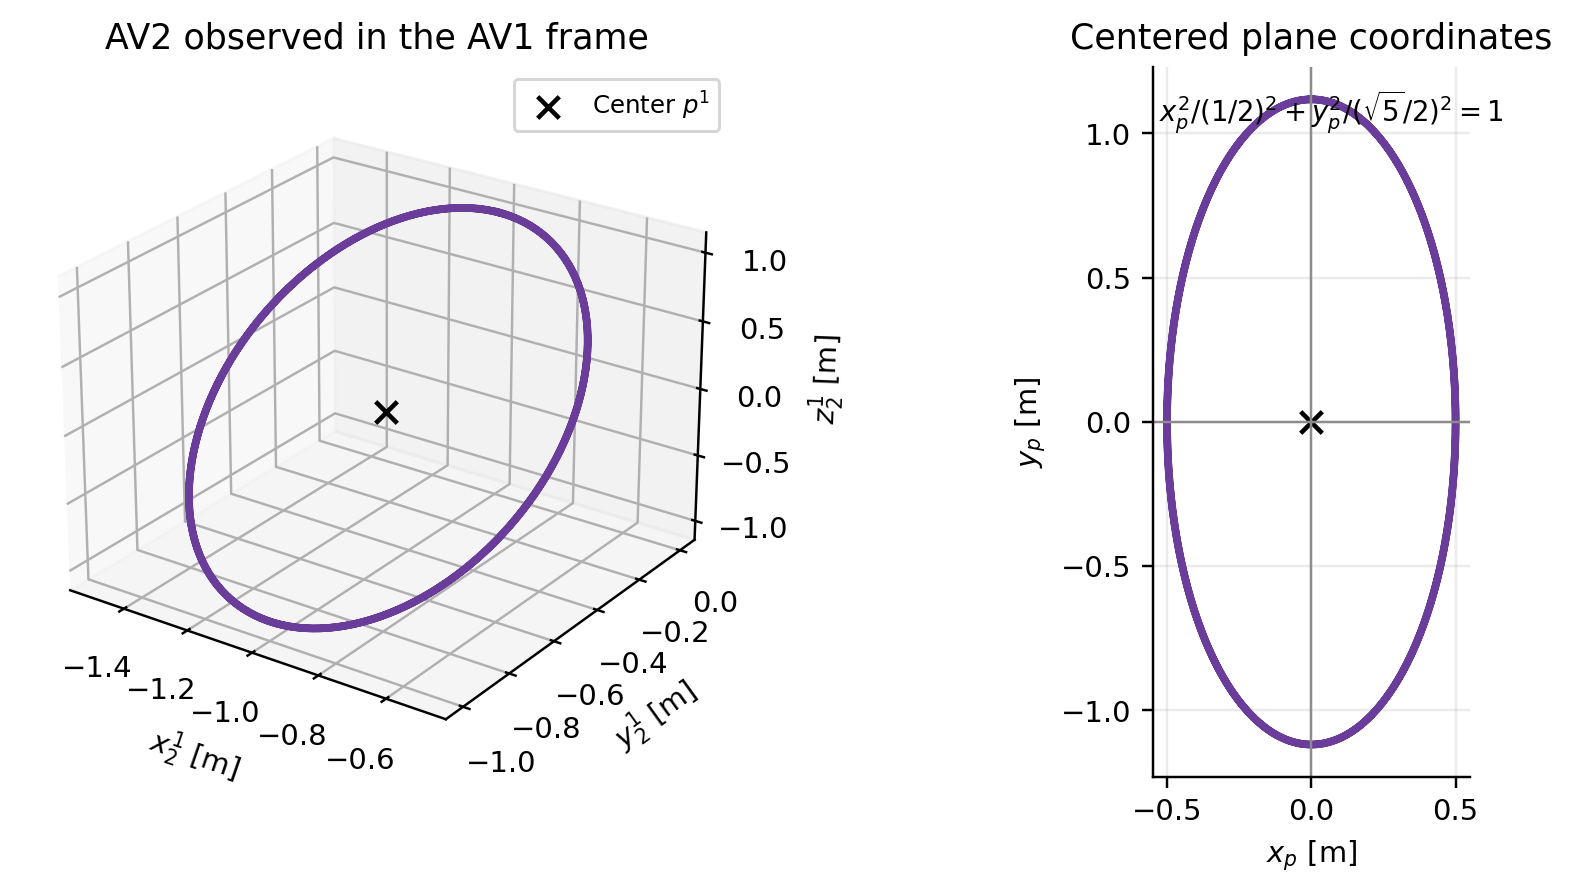
\includegraphics[width=0.96\textwidth]{figures/relative_trajectory.png}
\caption{Relative trajectory of AV2: an ellipse lying on $2y_2^1-z_2^1+1=0$.}
\label{fig:relative}
\end{figure}

\section{Quaternion Operator Properties}

For a quaternion $\vect{q}=[q_1,q_2,q_3,q_4]^{\mathsf T}$, the assignment defines left- and right-product matrices $\Omega_1(\vect{q})$ and $\Omega_2(\vect{q})$ such that
\begin{equation}
\vect{q}_a\otimes\vect{q}_b
=\Omega_1(\vect{q}_a)\vect{q}_b
=\Omega_2(\vect{q}_b)\vect{q}_a.
\end{equation}

\subsection{Orthogonality for a unit quaternion}

Quaternion norms are multiplicative:
$\|\vect{q}\otimes\vect{x}\|=\|\vect{q}\|\,\|\vect{x}\|$. If $\|\vect{q}\|=1$, then left multiplication and right multiplication preserve the Euclidean norm of every $\vect{x}\in\R^4$. A linear map preserves all Euclidean norms exactly when its matrix is orthogonal. Consequently,
\begin{equation}
\Omega_i(\vect{q})^{\mathsf T}\Omega_i(\vect{q})
=\Omega_i(\vect{q})\Omega_i(\vect{q})^{\mathsf T}=I_4,
\qquad i\in\{1,2\}.
\end{equation}
The same result follows by direct multiplication: each diagonal entry is $\|\vect{q}\|^2=1$, while all cross terms cancel.

\subsection{Mapping to the identity quaternion}

For a unit quaternion, the inverse is the conjugate $\vect{q}^{-1}=\vect{q}^{*}$. The transpose product matrices implement multiplication by this inverse. Hence
\begin{equation}
\Omega_1(\vect{q})^{\mathsf T}\vect{q}
=\vect{q}^{-1}\otimes\vect{q}
=\begin{bmatrix}0&0&0&1\end{bmatrix}^{\mathsf T},
\end{equation}
and similarly
\begin{equation}
\Omega_2(\vect{q})^{\mathsf T}\vect{q}
=\vect{q}\otimes\vect{q}^{-1}
=\begin{bmatrix}0&0&0&1\end{bmatrix}^{\mathsf T}.
\end{equation}

\subsection{Commutation of left and right multiplication}

For arbitrary $\vect{x},\vect{y},\vect{z}\in\R^4$, associativity of the quaternion product gives
\begin{align}
\Omega_1(\vect{x})\Omega_2(\vect{y})\vect{z}
&=\vect{x}\otimes(\vect{z}\otimes\vect{y})\\
&=(\vect{x}\otimes\vect{z})\otimes\vect{y}\\
&=\Omega_2(\vect{y})\Omega_1(\vect{x})\vect{z}.
\end{align}
Since this holds for every $\vect{z}$,
$\Omega_1(\vect{x})\Omega_2(\vect{y})
=\Omega_2(\vect{y})\Omega_1(\vect{x})$.
Furthermore $\Omega_2(\vect{y})^{\mathsf T}=\Omega_2(\vect{y}^{*})$. Applying the preceding identity to $\vect{y}^{*}$ proves
\begin{equation}
\Omega_1(\vect{x})\Omega_2(\vect{y})^{\mathsf T}
=\Omega_2(\vect{y})^{\mathsf T}\Omega_1(\vect{x}).
\end{equation}

\section{Optional: Intrinsic and Extrinsic Rotations}

Let $R$ map body-frame coordinates into the world frame. A rotation $A$ about a fixed world axis pre-multiplies the current attitude, $R' = AR$. A rotation about the corresponding current body axis post-multiplies it, $R'=RA$. Starting from $I$, an extrinsic sequence $A_0,A_1,\ldots,A_n$ produces
\begin{equation}
R_{\mathrm{ext}}=A_nA_{n-1}\cdots A_1A_0.
\end{equation}
Applying the reversed sequence $A_n,A_{n-1},\ldots,A_0$ intrinsically produces
\begin{equation}
R_{\mathrm{int}}=I\,A_nA_{n-1}\cdots A_1A_0
=R_{\mathrm{ext}}.
\end{equation}
Therefore a fixed-axis sequence is equivalent to the reversed moving-axis sequence, independently of the selected axes, angles, or number of rotations.

\section{Discussion}

The experiment demonstrates why TF2 is more useful than manually recomputing every relative pose in each consumer. The frame publisher specifies only the world poses; TF2 composes, inverts, time-stamps, and stores these transforms so that the plotting node can request AV2 directly in AV1. The separation also makes the visualization node independent of the particular trajectory generator.

The numerical errors are at floating-point round-off scale because the validator and publisher evaluate equivalent closed-form expressions at synchronized transform times. This test verifies the implemented kinematics and transform direction, but it does not model network delay, sensor noise, clock disagreement, or real quadrotor dynamics. The specified trajectories are kinematic visualization examples rather than dynamically feasible flight commands.

\section{Conclusion}

The ROS Noetic workspace, package build, static computation graph, dynamic TF broadcaster, relative-transform listener, and RViz visualization were completed successfully. The observed graph and topic connections matched the launch design. The measured publication rate met the 50~Hz target, and all 40 synchronized samples passed the $10^{-3}$ validation limit with errors below $10^{-15}$. Analytical derivations confirmed the world-frame parabola, the AV1-frame oblique ellipse, the quaternion operator identities, and the intrinsic/extrinsic rotation equivalence.

\begin{thebibliography}{9}
\bibitem{mitlab2}
MIT SPARK Lab, ``LAB2 Exercises: ROS and Two-Drone Coordinate Frames,''
Visual Navigation for Autonomous Vehicles, 2023.
\url{https://vnav.mit.edu/labs_2023/lab2/exercises.html}

\bibitem{vnavrepo}
MIT SPARK Lab, ``VNAV-labs: Labs for MIT 16.485,'' GitHub repository.
\url{https://github.com/MIT-SPARK/VNAV-labs}

\bibitem{rep103}
T. Foote and M. Purvis, ``REP 103: Standard Units of Measure and Coordinate Conventions,'' Open Robotics.
\url{https://www.ros.org/reps/rep-0103.html}

\bibitem{tf2api}
Open Robotics, ``tf2\_ros TransformBroadcaster API, ROS Noetic.''
\url{https://docs.ros.org/en/noetic/api/tf2_ros/html/c++/classtf2__ros_1_1TransformBroadcaster.html}
\end{thebibliography}

\end{document}
